% Capitolul 8: Extensii Moderne ale Seriilor de Timp
% Prezentare academică de calitate Harvard
% Program de licență, Academia de Studii Economice din București

\documentclass[9pt, aspectratio=169, t]{beamer}

% Asigură încadrarea conținutului pe diapozitive
\setbeamersize{text margin left=8mm, text margin right=8mm}

%=============================================================================
% CONFIGURARE TEMĂ ȘI STIL
%=============================================================================
\usetheme{default}
% Utilizăm tema implicită pentru control curat al antetului/subsolului

% Paletă de Culori (potrivită cu PDF-ul Redispatch)
\definecolor{MainBlue}{RGB}{26, 58, 110}
\definecolor{AccentBlue}{RGB}{26, 58, 110}
\definecolor{IDAred}{RGB}{205, 0, 0}
\definecolor{DarkGray}{RGB}{51, 51, 51}
\definecolor{MediumGray}{RGB}{128, 128, 128}
\definecolor{LightGray}{RGB}{248, 248, 248}
\definecolor{VeryLightGray}{RGB}{235, 235, 235}
\definecolor{KeynoteGray}{RGB}{218, 218, 218}
\definecolor{SectionGray}{RGB}{120, 120, 120}
\definecolor{FooterGray}{RGB}{100, 100, 100}
\definecolor{Crimson}{RGB}{220, 53, 69}
\definecolor{Forest}{RGB}{46, 125, 50}
\definecolor{Amber}{RGB}{181, 133, 63}
\definecolor{Orange}{RGB}{230, 126, 34}
\definecolor{Purple}{RGB}{142, 68, 173}

% Fundal gradient (gradient Keynote exact 315°: alb la RGB 218,218,218)
\setbeamertemplate{background}{%
    \begin{tikzpicture}[remember picture, overlay]
        \shade[shading=axis, shading angle=315,
        top color=white, bottom color=KeynoteGray]
        (current page.south west) rectangle (current page.north east);
    \end{tikzpicture}%
}
% Culoare solidă de rezervă pentru compatibilitate
\setbeamercolor{background canvas}{bg=}

\setbeamercolor{palette primary}{bg=MainBlue, fg=white}
\setbeamercolor{palette secondary}{bg=MainBlue!85, fg=white}
\setbeamercolor{palette tertiary}{bg=MainBlue!70, fg=white}
\setbeamercolor{structure}{fg=MainBlue}
\setbeamercolor{title}{fg=IDAred}
\setbeamercolor{frametitle}{fg=IDAred, bg=}
\setbeamercolor{block title}{bg=MainBlue, fg=white}
\setbeamercolor{block body}{bg=VeryLightGray, fg=DarkGray}
\setbeamercolor{block title alerted}{bg=Crimson, fg=white}
\setbeamercolor{block body alerted}{bg=Crimson!8, fg=DarkGray}
\setbeamercolor{block title example}{bg=Forest, fg=white}
\setbeamercolor{block body example}{bg=Forest!8, fg=DarkGray}
\setbeamercolor{item}{fg=MainBlue}

% Culori subsol (suprascriu albastrul temei Madrid)
\setbeamercolor{author in head/foot}{fg=FooterGray, bg=}
\setbeamercolor{title in head/foot}{fg=FooterGray, bg=}
\setbeamercolor{date in head/foot}{fg=FooterGray, bg=}
\setbeamercolor{section in head/foot}{fg=FooterGray, bg=}
\setbeamercolor{subsection in head/foot}{fg=FooterGray, bg=}

% Stiluri marcatori (se aplică peste tot inclusiv în blocuri)
\setbeamertemplate{itemize item}{\color{MainBlue}$\boxdot$}
\setbeamertemplate{itemize subitem}{\color{MainBlue}$\blacktriangleright$}
\setbeamertemplate{itemize subsubitem}{\color{MainBlue}\tiny$\bullet$}
\setbeamertemplate{itemize/enumerate body begin}{\normalsize}
\setbeamertemplate{itemize/enumerate subbody begin}{\normalsize}

% Item spacing - compact style
\setlength{\leftmargini}{10pt}       % Level 1: minimal indent
\setlength{\leftmarginii}{10pt}      % Level 2: minimal additional indent
% Compact list spacing (zero extra space before/after lists in blocks)
\makeatletter
\def\@listi{\leftmargin\leftmargini \topsep 0pt \parsep 0pt \itemsep 0pt}
\def\@listii{\leftmargin\leftmarginii \topsep 0pt \parsep 0pt \itemsep 0pt}
\makeatother

\setbeamertemplate{navigation symbols}{}

%=============================================================================
% ANTET PERSONALIZAT
%=============================================================================
\setbeamertemplate{headline}{%
    \vskip10pt%
    \hbox to \paperwidth{%
        \hskip0.5cm%
        {\small\color{FooterGray}\renewcommand{\hyperlink}[2]{##2}\insertsectionhead}%
        \hfill%
        \textcolor{FooterGray}{\small\insertframenumber}%
        \hskip0.5cm%
    }%
    \vskip4pt%
    {\color{FooterGray}\hrule height 0.4pt}%
}

%=============================================================================
% CUSTOM FOOTER
%=============================================================================
\usepackage{fontawesome5}

\setbeamertemplate{footline}{%
    {\color{FooterGray}\hrule height 0.4pt}%
    \vskip4pt%
    \hbox to \paperwidth{%
        \hskip0.5cm%
        \textcolor{FooterGray}{\small Analiza și Prognoza Seriilor de Timp}%
        \hfill%
        \raisebox{-0.1em}{%
            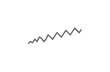
\begin{tikzpicture}[x=0.08em, y=0.08em, line width=0.4pt]
                \draw[FooterGray] (0,3) -- (1,4) -- (2,3.5) -- (3,5) -- (4,4) -- (5,6) -- (6,5.5) -- (7,4) -- (8,5) -- (9,7) -- (10,6) -- (11,5) -- (12,6.5) -- (13,8) -- (14,7) -- (15,6) -- (16,7.5) -- (17,9) -- (18,8) -- (19,7) -- (20,8.5) -- (21,10) -- (22,9) -- (23,8) -- (24,9.5);
            \end{tikzpicture}%
        }%
        \hskip0.5cm%
    }%
    \vskip6pt%
}

%=============================================================================
% PACHETE
%=============================================================================
\usepackage[utf8]{inputenc}
\usepackage[T1]{fontenc}
\usepackage{amsmath, amssymb, amsthm}
\usepackage{mathtools}
\usepackage{bm}
\usepackage{tikz}
\usetikzlibrary{arrows.meta, positioning, shapes, calc, decorations.pathreplacing, shadings}
\usepackage{booktabs}
\usepackage{multirow}
\usepackage{array}
\usepackage{graphicx}
\usepackage{hyperref}
\usepackage{colortbl}
\hypersetup{colorlinks=true, linkcolor=MainBlue, urlcolor=MainBlue}
\graphicspath{{../../logos/}{../../charts/}{../../photos/}}
\hfuzz=2pt  % Suppress tiny overfull warnings (<2pt)
\vfuzz=2pt  % Suppress tiny vertical overfull warnings (<2pt)

%=============================================================================
% COMANDA QUANTLET
%=============================================================================
\newcommand{\quantlet}[2]{%
    \hfill\href{#2}{%
        \raisebox{-0.15em}{\includegraphics[height=0.7em]{ql_logo.png}}%
        \textcolor{MainBlue}{\tiny\ #1}%
    }%
}

%=============================================================================
% MEDII PENTRU TEOREME
%=============================================================================
\theoremstyle{definition}
\setbeamertemplate{theorems}[numbered]
\newtheorem{defn}{Definiție}
\newtheorem{thm}{Teoremă}
\newtheorem{prop}{Propoziție}
\newtheorem{rmk}{Observație}

%=============================================================================
% CENTRED MINIPAGE (fără spațiu vertical suplimentar)
%=============================================================================
\newenvironment{cminipage}[1]{%
    \par\noindent\hfill\begin{minipage}{#1}\ignorespaces
}{%
    \end{minipage}\hfill\null\par
}

%=============================================================================
% COMENZI PERSONALIZATE
%=============================================================================
\newcommand{\E}{\mathbb{E}}
\newcommand{\Var}{\text{Var}}
\newcommand{\Cov}{\text{Cov}}
\newcommand{\Corr}{\text{Corr}}
\newcommand{\R}{\mathbb{R}}
\newcommand{\N}{\mathbb{N}}
\newcommand{\Z}{\mathbb{Z}}
\newcommand{\B}{\mathbf{B}}
\newcommand{\imark}{\textcolor{MainBlue}{\textbullet}}
\newcommand{\RMSE}{\text{RMSE}}
\newcommand{\MAE}{\text{MAE}}
\newcommand{\MAPE}{\text{MAPE}}

%=============================================================================
% PAGINĂ TITLU PERSONALIZATĂ
%=============================================================================
\defbeamertemplate*{title page}{hybrid}[1][]
{
    \vspace{0.2cm}
    % Rând logo-uri - antet superior (cu linkuri clickabile)
    \begin{center}
        \href{https://www.ase.ro}{\includegraphics[height=1.0cm]{ase_logo.png}}\hspace{0.3cm}%
        \href{https://theida.net}{\includegraphics[height=1.0cm]{ida_logo.png}}\hspace{0.3cm}%
        \href{https://blockchain-research-center.com}{\includegraphics[height=1.0cm]{brc_logo.png}}\hspace{0.3cm}%
        \href{https://www.ai4efin.ase.ro}{\includegraphics[height=1.0cm]{ai4efin_logo.png}}\hspace{0.3cm}%
        \href{https://ipe.ro/new}{\includegraphics[height=1.0cm]{acad_logo.png}}\hspace{0.3cm}%
        \href{https://www.digital-finance-msca.com}{\includegraphics[height=1.0cm]{msca_logo.png}}%
    \end{center}

    \vspace{0.6cm}

    % Titlu principal cu logo-uri Q pe părți (cu linkuri clickabile)
    \begin{center}
        \begin{minipage}{0.1\textwidth}
            \centering
            \href{https://quantlet.com}{\includegraphics[height=1.1cm]{ql_logo.png}}
        \end{minipage}%
        \begin{minipage}{0.78\textwidth}
            \centering
            {\LARGE\bfseries\usebeamercolor[fg]{title}\inserttitle}

            \vspace{0.3cm}

            {\usebeamerfont{subtitle}\usebeamercolor[fg]{title}\insertsubtitle}
        \end{minipage}%
        \begin{minipage}{0.1\textwidth}
            \centering
            \href{https://quantinar.com}{\includegraphics[height=1.1cm]{qr_logo.png}}
        \end{minipage}
    \end{center}

    \vspace{0.6cm}

    % Autori (aliniere la stânga)
    \hspace{0.5cm}{\usebeamerfont{author}\insertauthor}

    \vspace{0.3cm}

    % Institut/Afilieri (aliniere la stânga)
    \hspace{0.5cm}\begin{minipage}[t]{0.9\textwidth}
        \raggedright\small\insertinstitute
    \end{minipage}
}

%=============================================================================
% INFORMAȚII TITLU
%=============================================================================
\title[Analiza Seriilor de Timp]{Analiza și Prognoza Seriilor de Timp}
\subtitle{Capitolul 8: Extensii Moderne}
\author[D.T. Pele]{Daniel Traian PELE}
\institute{Academia de Studii Economice din București\\
IDA Institute Digital Assets\\
Blockchain Research Center\\
AI4EFin Artificial Intelligence for Energy Finance\\
Academia Română, Institutul de Prognoză Economică\\
MSCA Digital Finance}
\date{}

\begin{document}

% Pagina de titlu (fără antet/subsol)
{
\setbeamertemplate{headline}{}
\setbeamertemplate{footline}{}
\begin{frame}
    \titlepage
\end{frame}
}

%=============================================================================
% OBIECTIVE DE ÎNVĂȚARE
%=============================================================================
\begin{frame}{Obiective de învățare}
    \begin{cminipage}{0.95\textwidth}
        \begin{block}{La finalul acestui capitol, veți fi capabili să:}
            \begin{itemize}\setlength{\itemsep}{2pt}
                \item[\textcolor{MainBlue}{\textbf{1.}}] \textbf{Înțelegeți} conceptul de memorie lungă în seriile de timp
                \item[\textcolor{MainBlue}{\textbf{2.}}] \textbf{Estimați} și interpretați modele ARFIMA (AutoRegressive Fractionally Integrated Moving Average)
                \item[\textcolor{MainBlue}{\textbf{3.}}] \textbf{Aplicați} Random Forest (RF -- ansamblu de arbori de decizie) pentru prognoză seriilor de timp
                \item[\textcolor{MainBlue}{\textbf{4.}}] \textbf{Construiți} rețele LSTM (Long Short-Term Memory) pentru serii temporale
                \item[\textcolor{MainBlue}{\textbf{5.}}] \textbf{Comparați} performanța modelelor clasice vs ML (Machine Learning)
                \item[\textcolor{MainBlue}{\textbf{6.}}] \textbf{Alegeți} metoda potrivită în funcție de context
                \item[\textcolor{MainBlue}{\textbf{7.}}] \textbf{Implementați} aceste metode în Python
            \end{itemize}
        \end{block}
    \end{cminipage}
\end{frame}

%=============================================================================
% CUPRINS
%=============================================================================
\begin{frame}{Cuprins}
    \setbeamertemplate{section in toc}{\color{MainBlue}$\boxdot$~\inserttocsection}
    \tableofcontents
\end{frame}

%=============================================================================
\section{Motivație}
%=============================================================================

\begin{frame}{De la modele clasice la machine learning}
    \begin{cminipage}{0.95\textwidth}
        \begin{block}{Limitările modelelor ARIMA (AutoRegressive Integrated Moving Average)}
            \begin{itemize}\setlength{\itemsep}{0pt}
                \item Presupun \textbf{memorie scurtă}: autocorelațiile scad exponențial
                \item Relații \textbf{liniare} între variabile
                \item Dificultăți cu \textbf{pattern-uri complexe} și neliniare
                \item Necesită \textbf{staționaritate} (prin diferențiere)
            \end{itemize}
        \end{block}

        \vspace{0.2cm}

        \begin{alertblock}{Soluții moderne}
            \begin{itemize}\setlength{\itemsep}{0pt}
                \item \textbf{ARFIMA}: Captează memoria lungă (autocorelații care scad lent)
                \item \textbf{Random Forest}: Relații neliniare, robustețe la outlieri
                \item \textbf{LSTM}: Pattern-uri secvențiale complexe, dependențe pe termen lung
            \end{itemize}
        \end{alertblock}
    \end{cminipage}
\end{frame}

\begin{frame}{Când să folosim fiecare metodă?}
    \begin{cminipage}{0.95\textwidth}
        \begin{center}
            \begin{tabular}{l|c|c|c|c}
                \toprule
                \textbf{Caracteristică} & \textbf{ARIMA} & \textbf{ARFIMA} & \textbf{RF} & \textbf{LSTM} \\
                \midrule
                Memorie lungă & $\times$ & $\checkmark$ & $\checkmark$ & $\checkmark$ \\
                Relații neliniare & $\times$ & $\times$ & $\checkmark$ & $\checkmark$ \\
                Interpretabilitate & $\checkmark$ & $\checkmark$ & $\sim$ & $\times$ \\
                Date puține & $\checkmark$ & $\checkmark$ & $\times$ & $\times$ \\
                Variabile exogene & $\checkmark$ & $\checkmark$ & $\checkmark$ & $\checkmark$ \\
                Incertitudine & $\checkmark$ & $\checkmark$ & $\sim$ & $\times$ \\
                \bottomrule
            \end{tabular}
        \end{center}

        \vspace{0.1cm}

        \begin{exampleblock}{Regula de aur}
            \begin{itemize}\setlength{\itemsep}{0pt}
                \item Începe \textbf{simplu} (ARIMA), apoi crește complexitatea doar dacă este justificat de date și performanță.
            \end{itemize}
        \end{exampleblock}
    \end{cminipage}
\end{frame}

%=============================================================================
\section{ARFIMA: Modele cu Memorie lungă}
%=============================================================================

\begin{frame}{Comparație ACF (Funcția de Autocorelație): memorie scurtă vs lungă}
    \vspace{-0.2cm}
    {\footnotesize
    \begin{block}{Interpretare}
        \begin{itemize}\setlength{\itemsep}{0pt}
            \item \textbf{Date}: AR(1) simulat cu $\phi=0.8$ și ARFIMA(0,$d$,0) cu $d=0.35$ ($n=1000$)
            \item \textbf{Stânga}: AR(1) --- autocorelații care scad exponențial (memorie scurtă)
            \item \textbf{Dreapta}: ARFIMA cu $d=0.35$ --- autocorelații care scad hiperbolic (memorie lungă)
        \end{itemize}
    \end{block}
    }
    \begin{center}
        \includegraphics[width=0.95\textwidth, height=0.50\textheight, keepaspectratio]{ch8_acf_comparison.pdf}
    \end{center}
    \quantlet{TSA\_ch8\_acf\_comparison}{https://github.com/QuantLet/TSA/tree/main/TSA_ch8/TSA_ch8_acf_comparison}
\end{frame}

\begin{frame}{Ce este memoria lungă?}
    \begin{cminipage}{0.95\textwidth}
        \begin{block}{Memorie scurtă (ARMA)}
            \begin{itemize}\setlength{\itemsep}{0pt}
                \item Autocorelațiile $\rho_k$ scad \textbf{exponențial}: $|\rho_k| \leq C \cdot r^k$, $r < 1$
                \item Efectele șocurilor dispar \textbf{rapid}
                \item Sumă finită: $\sum_{k=0}^{\infty} |\rho_k| < \infty$
            \end{itemize}
        \end{block}

        \vspace{0.1cm}

        \begin{alertblock}{Memorie lungă (ARFIMA)}
            \begin{itemize}\setlength{\itemsep}{0pt}
                \item Autocorelațiile scad \textbf{hiperbolic}: $\rho_k \sim C \cdot k^{2d-1}$
                \item Efectele șocurilor persistă \textbf{mult timp}
                \item Sumă infinită: $\sum_{k=0}^{\infty} |\rho_k| = \infty$ (pentru $d > 0$)
            \end{itemize}
        \end{alertblock}

        \vspace{0.1cm}

        \begin{exampleblock}{Exemple cu memorie lungă}
            \begin{itemize}\setlength{\itemsep}{0pt}
                \item Volatilitatea piețelor financiare, debite râuri, trafic rețea, inflație
            \end{itemize}
        \end{exampleblock}
    \end{cminipage}
\end{frame}

\begin{frame}{Modelul ARFIMA(p,d,q)}
    \begin{cminipage}{0.95\textwidth}
        \vspace{-0.3cm}
        {\small
        \begin{defn}[ARFIMA]
            \begin{itemize}\setlength{\itemsep}{0pt}
                \item \textbf{Model}: Un proces $\{Y_t\}$ urmează un model \textbf{ARFIMA(p,d,q)} dacă:
                $\phi(L)(1-L)^d Y_t = \theta(L)\varepsilon_t$
                \item \textbf{Parametru}: $d \in (-0.5, 0.5)$ este parametrul de \textbf{diferențiere fracționară}
            \end{itemize}
        \end{defn}
        }
        \vspace{-0.1cm}
        {\footnotesize
        \begin{block}{Operatorul de diferențiere fracționară}
            \begin{itemize}\setlength{\itemsep}{0pt}
                \item $(1-L)^d = \sum_{k=0}^{\infty} \binom{d}{k}(-L)^k = 1 - dL - \frac{d(1-d)}{2!}L^2 - \cdots$
            \end{itemize}
        \end{block}
        }
        \vspace{-0.1cm}
        {\scriptsize
        \begin{block}{Cazuri particulare}
            \begin{itemize}\setlength{\itemsep}{0pt}
                \item $d = 0$: ARMA standard (memorie scurtă)
                \item $0 < d < 0.5$: Memorie lungă, staționaritate
                \item $d = 0.5$: Limita staționarității
                \item $0.5 \leq d < 1$: Nestaționaritate, dar mean-reverting
                \item $d = 1$: Random walk (ARIMA standard)
            \end{itemize}
        \end{block}
        }
    \end{cminipage}
\end{frame}

\begin{frame}{Efectul parametrului $d$ asupra ACF}
    \vspace{-0.2cm}
    {\footnotesize
    \begin{block}{Interpretare}
        \begin{itemize}\setlength{\itemsep}{0pt}
            \item \textbf{Date}: ARFIMA(0,$d$,0) simulat pentru $d \in \{0.1, 0.2, 0.3, 0.4\}$ ($n=1000$)
            \item Cu cât $d$ este mai mare, cu atât autocorelațiile scad mai lent
            \item Pentru $d \to 0.5$, autocorelațiile rămân semnificative chiar și la lag-uri foarte mari
        \end{itemize}
    \end{block}
    }
    \begin{center}
        \includegraphics[width=0.95\textwidth, height=0.50\textheight, keepaspectratio]{ch8_arfima_d_effect.pdf}
    \end{center}
    \quantlet{TSA\_ch8\_arfima\_d\_effect}{https://github.com/QuantLet/TSA/tree/main/TSA_ch8/TSA_ch8_arfima_d_effect}
\end{frame}

\begin{frame}{Interpretarea parametrului $d$}
    \begin{cminipage}{0.95\textwidth}
        \begin{center}
            \begin{tabular}{c|l|l}
                \toprule
                \textbf{Valoare $d$} & \textbf{Comportament ACF} & \textbf{Interpretare} \\
                \midrule
                $d = 0$ & Scădere exponențială & Memorie scurtă \\
                $0 < d < 0.5$ & Scădere hiperbolică & Memorie lungă, staționară \\
                $d = 0.5$ & ACF nesumabilă & La limită \\
                $0.5 < d < 1$ & Scădere foarte lentă & Memorie lungă, nestaționară \\
                $d = 1$ & ACF = 1 (constant) & Random walk \\
                \bottomrule
            \end{tabular}
        \end{center}

        \vspace{0.1cm}

        \begin{block}{Parametrul Hurst $H$}
            \begin{itemize}\setlength{\itemsep}{0pt}
                \item \textbf{Relația}: $d = H - 0.5$
                \begin{itemize}\setlength{\itemsep}{0pt}
                    \item $H = 0.5$: Mers aleator (fără memorie)
                    \item $H > 0.5$: Persistență (trend-following)
                    \item $H < 0.5$: Anti-persistență (mean-reverting)
                \end{itemize}
            \end{itemize}
        \end{block}
    \end{cminipage}
\end{frame}

\begin{frame}{Exponentul Hurst: interpretare vizuală}
    \vspace{-0.2cm}
    {\scriptsize
    \begin{block}{Interpretare}
        \begin{itemize}\setlength{\itemsep}{0pt}
            \item \textbf{Date}: Mișcare Browniană fracționară simulată cu $H \in \{0.3, 0.5, 0.7\}$
            \item \textbf{H $<$ 0.5}: Mean-reverting \quad \textbf{H = 0.5}: Mers aleator
            \item \textbf{H $>$ 0.5}: Persistentă (trend-following)
        \end{itemize}
    \end{block}
    }
    \begin{center}
        \includegraphics[width=0.95\textwidth, height=0.50\textheight, keepaspectratio]{ch8_hurst_interpretation.pdf}
    \end{center}
    \quantlet{TSA\_ch8\_hurst\_interpretation}{https://github.com/QuantLet/TSA/tree/main/TSA_ch8/TSA_ch8_hurst_interpretation}
\end{frame}

\begin{frame}{ARIMA vs ARFIMA: comparație simulată}
    \vspace{-0.2cm}
    {\footnotesize
    \begin{block}{Interpretare}
        \begin{itemize}\setlength{\itemsep}{0pt}
            \item \textbf{Date}: ARIMA(1,1,1) simulat vs ARFIMA(1,$d$,1) cu $d=0.35$
            \item \textbf{ARIMA} (stânga): ACF scade \textbf{exponențial} --- șocurile sunt ``uitate'' rapid
            \item \textbf{ARFIMA} (dreapta, $d=0.35$): ACF scade \textbf{hiperbolic} --- șocurile persistă mult timp
        \end{itemize}
    \end{block}
    }
    \begin{center}
        \includegraphics[width=0.95\textwidth, height=0.50\textheight, keepaspectratio]{ch8_arima_vs_arfima.pdf}
    \end{center}
    \quantlet{TSA\_ch8\_arima\_vs\_arfima}{https://github.com/QuantLet/TSA/tree/main/TSA_ch8/TSA_ch8_arima_vs_arfima}
\end{frame}

\begin{frame}{Exemplu date reale: analiza memoriei lungi EUR/RON}
    \vspace{-0.2cm}
    {\footnotesize
    \begin{block}{Interpretare}
        \begin{itemize}\setlength{\itemsep}{0pt}
            \item \textbf{Date}: Cursul zilnic EUR/RON (Yahoo Finance, 2015--2025)
            \item \textbf{Randamente}: $H \approx 0.50$, $d \approx 0$ --- memorie scurtă
            \item \textbf{Randamente pătrate}: $H \approx 0.65$, $d \approx 0.15$ --- memorie lungă în volatilitate
        \end{itemize}
    \end{block}
    }
    \begin{center}
        \includegraphics[width=0.95\textwidth, height=0.50\textheight, keepaspectratio]{ch8_eurron_long_memory.pdf}
    \end{center}
    \quantlet{TSA\_ch8\_eurron\_long\_memory}{https://github.com/QuantLet/TSA/tree/main/TSA_ch8/TSA_ch8_eurron_long_memory}
\end{frame}

\begin{frame}{Exemplu ARFIMA: Volatilitatea realizată S\&P 500}
    \vspace{-0.2cm}
    {\scriptsize
    \begin{block}{Rezultate estimare}
        \begin{itemize}\setlength{\itemsep}{0pt}
            \item \textbf{Date}: Randamentele zilnice S\&P 500 (Yahoo Finance, 2015--2024)
            \item Hurst: $H = 0.92$, $d = H - 0.5 = 0.42$ -- memorie lungă puternică
        \end{itemize}
    \end{block}
    \begin{alertblock}{Observație cheie}
        \begin{itemize}\setlength{\itemsep}{0pt}
            \item Volatilitatea are \textbf{memorie lungă} -- șocurile persistă mai mult decât în ARMA
            \item Folosiți ARFIMA sau FIGARCH (Fractionally Integrated GARCH)!
        \end{itemize}
    \end{alertblock}
    }
    \begin{center}
        \includegraphics[width=0.95\textwidth, height=0.42\textheight, keepaspectratio]{ch8_arfima_real_data.pdf}
    \end{center}
    \quantlet{TSA\_ch8\_arfima\_sp500}{https://github.com/QuantLet/TSA/tree/main/TSA_ch8/TSA_ch8_arfima_sp500}
\end{frame}

\begin{frame}{Estimarea parametrului $d$}
    \begin{cminipage}{0.95\textwidth}
        \begin{block}{Metode de estimare}
            \begin{itemize}\setlength{\itemsep}{0pt}
                \item \textbf{GPH (Geweke-Porter-Hudak)}: Regresie în domeniul frecvență
                \begin{itemize}\setlength{\itemsep}{0pt}
                    \item $\ln I(\omega_j) = c - d \cdot \ln\bigl(4\sin^2\frac{\omega_j}{2}\bigr) + \varepsilon_j$
                \end{itemize}
                \item \textbf{R/S (Rescaled Range)}: Metoda lui Hurst
                \begin{itemize}\setlength{\itemsep}{0pt}
                    \item $\frac{R}{S}(n) \sim c \cdot n^H$
                \end{itemize}
                \item \textbf{MLE (Maximum Likelihood)}: Estimare completă ARFIMA
                \item \textbf{Whittle}: Aproximare eficientă în domeniul frecvență
            \end{itemize}
        \end{block}

        \vspace{0.2cm}

        {\footnotesize
        \begin{exampleblock}{Implementare}
            \begin{itemize}\setlength{\itemsep}{0pt}
                \item În Python: pachetul \texttt{arch}, sau \texttt{statsmodels.tsa.arima.model.ARIMA}
                \item Se specifică \texttt{order=(p,d,q)} unde $d$ poate fi fracționar
            \end{itemize}
        \end{exampleblock}
        }
    \end{cminipage}
\end{frame}

\begin{frame}{Exemplu real: memorie lungă în volatilitate}
    \vspace{-0.2cm}
    {\scriptsize
    \begin{alertblock}{Notă}
        \begin{itemize}\setlength{\itemsep}{0pt}
            \item Estimarea ARFIMA necesită pachete specializate
            \item În practică, se folosește adesea \texttt{arch} sau \texttt{fracdiff} în Python
        \end{itemize}
    \end{alertblock}
    }
    \begin{center}
        \includegraphics[width=0.95\textwidth, height=0.50\textheight, keepaspectratio]{ch8_volatility_long_memory.pdf}
    \end{center}
    \quantlet{TSA\_ch8\_volatility\_long\_memory}{https://github.com/QuantLet/TSA/tree/main/TSA_ch8/TSA_ch8_volatility_long_memory}
\end{frame}

%=============================================================================
\section{Random Forest pentru serii de timp}
%=============================================================================

\begin{frame}{Random Forest: concepte de bază}
    \begin{cminipage}{0.95\textwidth}
        \begin{block}{Ce este Random Forest?}
            \begin{itemize}\setlength{\itemsep}{0pt}
                \item \textbf{Ansamblu} de arbori de decizie
                \item Fiecare arbore antrenat pe un \textbf{subset bootstrap} al datelor
                \item La fiecare nod, se selectează \textbf{aleator} un subset de features
                \item Predicția finală = \textbf{media} predicțiilor tuturor arborilor
            \end{itemize}
        \end{block}

        \vspace{0.2cm}

        \begin{exampleblock}{Avantaje pentru serii de timp}
            \begin{itemize}\setlength{\itemsep}{0pt}
                \item Captează \textbf{relații neliniare}
                \item \textbf{Robust} la outlieri și zgomot
                \item Nu necesită \textbf{staționaritate}
                \item Oferă \textbf{importanța features} (interpretabilitate)
                \item Funcționează bine cu \textbf{multe variabile}
            \end{itemize}
        \end{exampleblock}
    \end{cminipage}
\end{frame}

\begin{frame}{Feature engineering: ilustrare}
    \vspace{-0.2cm}
    {\footnotesize
    \begin{block}{Interpretare}
        \begin{itemize}\setlength{\itemsep}{0pt}
            \item \textbf{Date}: Consum zilnic de electricitate Germania (OPSD -- Open Power System Data, 2012--2017)
            \item Transformăm seria temporală în features: lag-uri, statistici rolling
            \item Modelul RF învață relațiile dintre acestea și valorile viitoare
        \end{itemize}
    \end{block}
    }
    \begin{center}
        \includegraphics[width=0.95\textwidth, height=0.50\textheight, keepaspectratio]{ch8_feature_engineering.pdf}
    \end{center}
    \quantlet{TSA\_ch8\_feature\_engineering}{https://github.com/QuantLet/TSA/tree/main/TSA_ch8/TSA_ch8_feature_engineering}
\end{frame}

\begin{frame}{Pregătirea datelor pentru Random Forest}
    \begin{cminipage}{0.95\textwidth}
        \begin{block}{Feature Engineering pentru serii de timp}
            \begin{enumerate}\setlength{\itemsep}{0pt}
                \item \textbf{Lag features}: $Y_{t-1}, Y_{t-2}, \ldots, Y_{t-p}$
                \item \textbf{Rolling statistics}: medie mobilă, deviație standard
                \item \textbf{Calendar features}: ziua săptămânii, luna, sezon
                \item \textbf{Trend features}: timp, trend pătratic
                \item \textbf{Variabile exogene}: indicători economici, evenimente
            \end{enumerate}
        \end{block}

        \vspace{0.2cm}

        \begin{alertblock}{Atenție: Data Leakage!}
            \begin{itemize}\setlength{\itemsep}{0pt}
                \item Nu folosi informații din viitor în features
                \item Train/test split: \textbf{temporal}, nu aleator!
                \item Rolling statistics: calculează doar pe date \textbf{anterioare}
            \end{itemize}
        \end{alertblock}
    \end{cminipage}
\end{frame}


\begin{frame}{Random Forest: exemplu de prognoză}
    \vspace{-0.2cm}
    {\scriptsize
    \begin{block}{Interpretare}
        \begin{itemize}\setlength{\itemsep}{0pt}
            \item \textbf{Date}: Consum zilnic de electricitate Germania (OPSD, 2012--2017)
            \item Modelul RF antrenat pe date istorice (albastru) produce prognoze (roșu punctat)
            \item Prognozele urmăresc bine valorile reale din perioada de test (verde)
        \end{itemize}
    \end{block}
    }
    \begin{center}
        \includegraphics[width=0.95\textwidth, height=0.50\textheight, keepaspectratio]{ch8_rf_prediction.pdf}
    \end{center}
    \quantlet{TSA\_ch8\_rf\_prediction}{https://github.com/QuantLet/TSA/tree/main/TSA_ch8/TSA_ch8_rf_prediction}
\end{frame}

\begin{frame}{Importanța features și interpretare}
    \begin{cminipage}{0.95\textwidth}
        \begin{block}{Feature importance}
            \begin{itemize}\setlength{\itemsep}{0pt}
                \item \textbf{Mean Decrease Impurity (MDI)}: Reducerea impurității la fiecare split
                \item \textbf{Permutation Importance}: Cât scade performanța când feature-ul e permutat aleator
            \end{itemize}
        \end{block}

        \vspace{0.2cm}

        \begin{block}{Interpretare tipică pentru serii de timp}
            \begin{itemize}\setlength{\itemsep}{0pt}
                \item \texttt{lag\_1} foarte important $\succ$ Autocorelare puternică
                \item \texttt{rolling\_mean} important $\succ$ Trend local contează
                \item \texttt{month} important $\succ$ Sezonalitate prezentă
            \end{itemize}
        \end{block}

        \vspace{0.2cm}

        {\footnotesize
        \begin{block}{Cod}
            \begin{itemize}\setlength{\itemsep}{0pt}
                \item \texttt{rf.feature\_importances\_} sau \texttt{permutation\_importance(rf, X\_test, y\_test)}
            \end{itemize}
        \end{block}
        }
    \end{cminipage}
\end{frame}

%=============================================================================
\section{LSTM: Deep Learning pentru serii de timp}
%=============================================================================

\begin{frame}{Portret de cercetător: Hochreiter \& Schmidhuber}
    \vspace{-0.5cm}
    \begin{columns}[T]
        \begin{column}{0.22\textwidth}
            \centering
            \includegraphics[width=0.95\textwidth, height=0.18\textheight, keepaspectratio]{photo_sepp_hochreiter.jpg}
            \\[0.03cm]
            {\tiny\textcolor{MediumGray}{Sepp Hochreiter (*1967)}}\\[0.01cm]
            \href{https://en.wikipedia.org/wiki/Sepp_Hochreiter}{\faWikipediaW\ \textcolor{MainBlue}{\tiny Wikipedia (en)}}
        \end{column}
        \begin{column}{0.76\textwidth}
            \begin{block}{Biografie}
                {\scriptsize \begin{itemize}\setlength{\itemsep}{0pt}
                    \item \textbf{Sepp Hochreiter}: informatician austriac, profesor la Johannes Kepler University Linz
                    \item Conducător al ELLIS (European Laboratory for Learning and Intelligent Systems) Unit Linz
                    \item \textbf{J\"{u}rgen Schmidhuber}: informatician germano-elvețian, Director Științific al IDSIA (Istituto Dalle Molle di Studi sull'Intelligenza Artificiale)
                    \item Împreună au rezolvat problema gradientului care dispare
                \end{itemize}}
            \end{block}
        \end{column}
    \end{columns}
    \vspace{-0.25cm}
    \begin{columns}[T]
        \begin{column}{0.22\textwidth}
            \centering
            \includegraphics[width=0.95\textwidth, height=0.18\textheight, keepaspectratio]{photo_juergen_schmidhuber.jpg}
            \\[0.03cm]
            {\tiny\textcolor{MediumGray}{J\"{u}rgen Schmidhuber (*1963)}}\\[0.01cm]
            \href{https://en.wikipedia.org/wiki/J\%C3\%BCrgen_Schmidhuber}{\faWikipediaW\ \textcolor{MainBlue}{\tiny Wikipedia (en)}}
        \end{column}
        \begin{column}{0.76\textwidth}
            \begin{exampleblock}{Contribuții principale}
                {\scriptsize
                \begin{itemize}\setlength{\itemsep}{0pt}
                    \item \textbf{Long Short-Term Memory} (LSTM, 1997) --- arhitectură recurentă cu porți
                    \item Rezolvă problema gradientului care dispare
                    \item \textbf{Analiza gradientului care dispare} (Hochreiter, 1991) --- identificarea problemei fundamentale
                    \item \textbf{Poarta forget} (Gers et al., 2000) --- extensie crucială pentru LSTM
                    \item Fundament pentru modelarea modernă a secvențelor în NLP (Natural Language Processing), voce și serii de timp
                \end{itemize}}
            \end{exampleblock}
        \end{column}
    \end{columns}
\end{frame}

\begin{frame}{De la neuronul biologic la cel artificial}
    \vspace{-0.2cm}
    {\scriptsize
    \begin{block}{Analogia}
        \begin{itemize}\setlength{\itemsep}{0pt}
            \item \textbf{Dendrite} $\succ$ \textbf{Intrări} $x_i$ \quad \textbf{Sinapse} $\succ$ \textbf{Ponderi} $w_i$
            \item \textbf{Soma} $\succ$ \textbf{Sumă + Activare} \quad \textbf{Axon} $\succ$ \textbf{Ieșire} $y$
        \end{itemize}
    \end{block}
    }
    \begin{center}
        \includegraphics[width=0.95\textwidth, height=0.50\textheight, keepaspectratio]{ch8_neuron_comparison.pdf}
    \end{center}
    \quantlet{TSA\_ch8\_neuron\_comparison}{https://github.com/QuantLet/TSA/tree/main/TSA_ch8/TSA_ch8_neuron_comparison}
\end{frame}

\begin{frame}{Rețele neuronale recurente -- RNN (Recurrent Neural Network)}
    \begin{block}{Ideea de bază}
        \begin{itemize}\setlength{\itemsep}{0pt}
            \item Rețele care procesează \textbf{secvențe} de date
            \item Au \textbf{memorie internă} (hidden state)
            \item Starea curentă depinde de input + starea anterioară
        \end{itemize}
    \end{block}

    \vspace{0.1cm}

    \begin{center}
        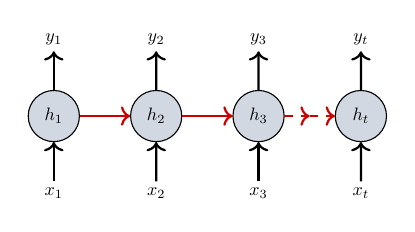
\begin{tikzpicture}[scale=0.65, transform shape]
        \node[draw, circle, minimum size=1cm, fill=MainBlue!20] (h1) at (0,0) {$h_1$};
        \node[draw, circle, minimum size=1cm, fill=MainBlue!20] (h2) at (2,0) {$h_2$};
        \node[draw, circle, minimum size=1cm, fill=MainBlue!20] (h3) at (4,0) {$h_3$};
        \node[draw, circle, minimum size=1cm, fill=MainBlue!20] (ht) at (6,0) {$h_t$};

        \node (x1) at (0,-1.5) {$x_1$};
        \node (x2) at (2,-1.5) {$x_2$};
        \node (x3) at (4,-1.5) {$x_3$};
        \node (xt) at (6,-1.5) {$x_t$};

        \node (y1) at (0,1.5) {$y_1$};
        \node (y2) at (2,1.5) {$y_2$};
        \node (y3) at (4,1.5) {$y_3$};
        \node (yt) at (6,1.5) {$y_t$};

        \draw[->, thick] (x1) -- (h1);
        \draw[->, thick] (x2) -- (h2);
        \draw[->, thick] (x3) -- (h3);
        \draw[->, thick] (xt) -- (ht);

        \draw[->, thick] (h1) -- (y1);
        \draw[->, thick] (h2) -- (y2);
        \draw[->, thick] (h3) -- (y3);
        \draw[->, thick] (ht) -- (yt);

        \draw[->, thick, IDAred] (h1) -- (h2);
        \draw[->, thick, IDAred] (h2) -- (h3);
        \draw[->, thick, IDAred, dashed] (h3) -- (5,0);
        \draw[->, thick, IDAred, dashed] (5,0) -- (ht);
    \end{tikzpicture}
    \end{center}

    \begin{alertblock}{Problema: Vanishing Gradient}
        \begin{itemize}\setlength{\itemsep}{0pt}
            \item RNN simple ``uită'' informația din trecut îndepărtat.
        \end{itemize}
    \end{alertblock}
\end{frame}

\begin{frame}{RNN desfășurată în timp}
    \begin{center}
        \includegraphics[width=0.95\textwidth, height=0.78\textheight, keepaspectratio]{ch8_rnn_unfolded.pdf}
    \end{center}
    \quantlet{TSA\_ch8\_rnn\_unfolded}{https://github.com/QuantLet/TSA/tree/main/TSA_ch8/TSA_ch8_rnn_unfolded}
\end{frame}

\begin{frame}{Celula LSTM: Diagrama detaliată}

    \vspace{-0.2cm}
    \begin{center}
        \includegraphics[width=0.95\textwidth, height=0.74\textheight, keepaspectratio]{ch8_lstm_cell.pdf}
    \end{center}
    \vspace{-0.3cm}
    {\footnotesize
    \begin{columns}[T]
        \begin{column}{0.32\textwidth}
            \begin{itemize}\setlength{\itemsep}{0pt}
                \item \textbf{Forget Gate} $f_t$
                \item $\sigma(W_f[h_{t-1}, x_t] + b_f)$
                \item Ce să uităm?
            \end{itemize}
        \end{column}
        \begin{column}{0.32\textwidth}
            \begin{itemize}\setlength{\itemsep}{0pt}
                \item \textbf{Input Gate} $i_t$
                \item $\sigma(W_i[h_{t-1}, x_t] + b_i)$
                \item Ce să stocăm?
            \end{itemize}
        \end{column}
        \begin{column}{0.32\textwidth}
            \begin{itemize}\setlength{\itemsep}{0pt}
                \item \textbf{Output Gate} $o_t$
                \item $\sigma(W_o[h_{t-1}, x_t] + b_o)$
                \item Ce să transmitem?
            \end{itemize}
        \end{column}
    \end{columns}
    }

    \quantlet{TSA\_ch8\_lstm\_cell}{https://github.com/QuantLet/TSA/tree/main/TSA_ch8/TSA_ch8_lstm_cell}
\end{frame}

\begin{frame}{LSTM: long short-term memory}
    \begin{cminipage}{0.95\textwidth}
        \vspace{-0.2cm}
        {\small
        \begin{block}{Soluția LSTM}
            \begin{itemize}\setlength{\itemsep}{0pt}
                \item \textbf{Concept}: Celule speciale cu 3 porți care controlează fluxul informației
                \item \textbf{Forget Gate} ($f_t$): Ce să uităm din memoria anterioară
                \item \textbf{Input Gate} ($i_t$): Ce informație nouă să adăugăm
                \item \textbf{Output Gate} ($o_t$): Ce să trimitem la ieșire
            \end{itemize}
        \end{block}

        \vspace{-0.05cm}

        \begin{block}{Ecuațiile LSTM}
            \begin{itemize}\setlength{\itemsep}{0pt}
                \item {\footnotesize
                \begin{align*}
            f_t &= \sigma(W_f \cdot [h_{t-1}, x_t] + b_f) & \text{(Forget)} \\
            i_t &= \sigma(W_i \cdot [h_{t-1}, x_t] + b_i) & \text{(Input)} \\
            \tilde{C}_t &= \tanh(W_C \cdot [h_{t-1}, x_t] + b_C) & \text{(Candidate)} \\
            C_t &= f_t \odot C_{t-1} + i_t \odot \tilde{C}_t & \text{(Cell state)} \\
            o_t &= \sigma(W_o \cdot [h_{t-1}, x_t] + b_o) & \text{(Output)} \\
            h_t &= o_t \odot \tanh(C_t) & \text{(Hidden state)}
        \end{align*}
                }
            \end{itemize}
        \end{block}
        }
    \end{cminipage}
\end{frame}

\begin{frame}{Arhitectura celulei LSTM}
    \vspace{-0.2cm}
    {\scriptsize
    \begin{block}{Interpretare}
        \begin{itemize}\setlength{\itemsep}{0pt}
            \item Porțile (forget, input, output) controlează ce informație este uitată, adăugată și transmisă
            \item \textbf{Cell state} permite gradienților să ``curgă'' fără degradare
        \end{itemize}
    \end{block}
    }
    \begin{center}
        \includegraphics[width=0.95\textwidth, height=0.50\textheight, keepaspectratio]{ch8_lstm_architecture.pdf}
    \end{center}
    \quantlet{TSA\_ch8\_lstm\_architecture}{https://github.com/QuantLet/TSA/tree/main/TSA_ch8/TSA_ch8_lstm_architecture}
\end{frame}

\begin{frame}{Avantajele LSTM pentru serii de timp}
    \begin{cminipage}{0.95\textwidth}
        \begin{exampleblock}{De ce LSTM?}
            \begin{itemize}\setlength{\itemsep}{0pt}
                \item Captează \textbf{dependențe pe termen lung} (spre deosebire de RNN simplu)
                \item Învață \textbf{pattern-uri complexe} și neliniare
                \item Gestionează \textbf{secvențe de lungimi variabile}
                \item Funcționează bine cu \textbf{date multivariate}
            \end{itemize}
        \end{exampleblock}

        \vspace{0.2cm}

        \begin{alertblock}{Dezavantaje}
            \begin{itemize}\setlength{\itemsep}{0pt}
                \item Necesită \textbf{multe date} pentru antrenare
                \item \textbf{Computațional intensiv}
                \item ``\textbf{Black box}'' - greu de interpretat
                \item Sensibil la \textbf{hiperparametri}
                \item Poate face \textbf{overfitting} ușor
            \end{itemize}
        \end{alertblock}
    \end{cminipage}
\end{frame}



%=============================================================================
\section{Comparație și Selecția modelului}
%=============================================================================

\begin{frame}{Time series cross-validation}
    \vspace{-0.2cm}
    {\footnotesize
    \begin{alertblock}{}
        \begin{itemize}\setlength{\itemsep}{0pt}
            \item \textbf{Important}: Setul de antrenare crește progresiv, testul este întotdeauna în viitor
        \end{itemize}
    \end{alertblock}
    }
    \begin{center}
        \includegraphics[width=0.95\textwidth, height=0.50\textheight, keepaspectratio]{ch8_timeseries_cv.pdf}
    \end{center}
    \quantlet{TSA\_ch8\_timeseries\_cv}{https://github.com/QuantLet/TSA/tree/main/TSA_ch8/TSA_ch8_timeseries_cv}
\end{frame}

\begin{frame}{Metrici de evaluare}
    \begin{cminipage}{0.95\textwidth}
        \begin{block}{Metrici comune}
            \begin{itemize}\setlength{\itemsep}{0pt}
                \item \textbf{RMSE} (Root Mean Squared Error): $\sqrt{\frac{1}{n}\sum_{i=1}^n (y_i - \hat{y}_i)^2}$ $\succ$ Eroare în unități originale
                \item \textbf{MAE} (Mean Absolute Error): $\frac{1}{n}\sum_{i=1}^n |y_i - \hat{y}_i|$ $\succ$ Robust la outlieri
                \item \textbf{MAPE} (Mean Absolute Percentage Error): $\frac{100}{n}\sum_{i=1}^n \left|\frac{y_i - \hat{y}_i}{y_i}\right|$ $\succ$ Eroare procentuală
                \item \textbf{MASE} (Mean Absolute Scaled Error): Comparat cu benchmark naiv
            \end{itemize}
        \end{block}

        \vspace{0.2cm}

        \begin{alertblock}{Validare pentru serii de timp}
            \begin{itemize}\setlength{\itemsep}{0pt}
                \item \textbf{Nu} folosiți cross-validation standard!
                \item Folosiți \textbf{Time series cross-validation} (walk-forward)
                \item Sau \textbf{train/validation/test} split temporal
            \end{itemize}
        \end{alertblock}
    \end{cminipage}
\end{frame}

\begin{frame}{Ghid de selecție a modelului}
    \vspace{-0.4cm}
    {\footnotesize
    \begin{center}
        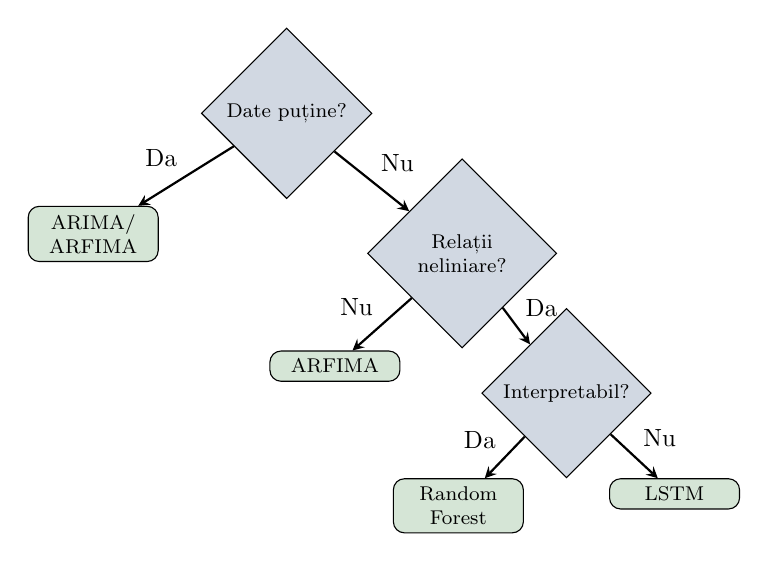
\begin{tikzpicture}[scale=0.9, transform shape,
        node distance=1.0cm,
        decision/.style={diamond, draw, fill=MainBlue!20, text width=2.0cm, align=center, inner sep=1pt, font=\footnotesize},
        block/.style={rectangle, draw, fill=Forest!20, text width=1.6cm, align=center, rounded corners, font=\footnotesize},
        arrow/.style={thick,->,>=stealth}
    ]
        \node[decision] (start) {Date puține?};
        \node[block, below left=0.7cm and 1.2cm of start] (arima) {ARIMA/ ARFIMA};
        \node[decision, below right=0.7cm and 1.2cm of start] (nonlin) {Relații neliniare?};
        \node[block, below left=0.7cm and 0.2cm of nonlin] (arfima) {ARFIMA};
        \node[decision, below right=0.7cm and 0.2cm of nonlin] (interp) {Interpretabil?};
        \node[block, below left=0.6cm and 0cm of interp] (rf) {Random Forest};
        \node[block, below right=0.6cm and 0cm of interp] (lstm) {LSTM};

        \draw[arrow] (start) -- node[above left] {Da} (arima);
        \draw[arrow] (start) -- node[above right] {Nu} (nonlin);
        \draw[arrow] (nonlin) -- node[above left] {Nu} (arfima);
        \draw[arrow] (nonlin) -- node[above right] {Da} (interp);
        \draw[arrow] (interp) -- node[above left] {Da} (rf);
        \draw[arrow] (interp) -- node[above right] {Nu} (lstm);
    \end{tikzpicture}
    \end{center}
    }
\end{frame}

%=============================================================================
\section{Aplicații practice}
%=============================================================================

\begin{frame}{Bitcoin: evoluția prețului și randamentele}
    \vspace{-0.2cm}
    {\footnotesize
    \begin{block}{Observații cheie}
        \begin{itemize}\setlength{\itemsep}{0pt}
            \item Creștere exponențială a prețului $\succ$ distribuție puternic \textbf{leptokurtotică}
            \item Randamentele zilnice: medie $\approx 0.15\%$, volatilitate $\approx 3.5\%$
            \item Volatility clustering evident $\succ$ perioadele de criză (2018, 2020, 2022)
            \item Kurtosis $\approx 10$--$15$ (mult peste 3 al normalei)
        \end{itemize}
    \end{block}
    }
    \begin{center}
        \includegraphics[width=0.95\textwidth, height=0.46\textheight, keepaspectratio]{ch10_bitcoin_overview.pdf}
    \end{center}
    \quantlet{TSA\_ch10\_btc\_returns}{https://github.com/QuantLet/TSA/tree/main/TSA_ch10/TSA_ch10_btc_returns}
\end{frame}

\begin{frame}{Studiu de caz: prognoza prețului Bitcoin}
    \begin{cminipage}{0.95\textwidth}
        \begin{block}{De ce Bitcoin?}
            \begin{itemize}\setlength{\itemsep}{0pt}
                \item Volatilitate \textbf{extremă} și pattern-uri complexe
                \item Potențială \textbf{memorie lungă} în volatilitate
                \item Relații \textbf{neliniare} cu variabile exogene
                \item Date disponibile la \textbf{frecvență înaltă}
            \end{itemize}
        \end{block}
        \vspace{0.1cm}
        \begin{exampleblock}{Abordare comparativă}
            \begin{enumerate}\setlength{\itemsep}{0pt}
                \item ARIMA pe randamente
                \item ARFIMA pentru memorie lungă
                \item Random Forest cu features tehnice
                \item LSTM pe secvențe de prețuri
            \end{enumerate}
        \end{exampleblock}
    \end{cminipage}
\end{frame}

\begin{frame}{Bitcoin: ACF și evidența pentru memorie lungă}
    \vspace{-0.2cm}
    {\footnotesize
    \begin{block}{Analiză ACF}
        \begin{itemize}\setlength{\itemsep}{0pt}
            \item ACF randamente: scădere rapidă $\succ$ memorie scurtă în medie
            \item ACF randamente pătrate: scădere \textbf{lentă, hiperbolică}
            \begin{itemize}\setlength{\itemsep}{0pt}
                \item[$\blacktriangleright$] Indică \textbf{memorie lungă în volatilitate}
                \item[$\blacktriangleright$] Hurst $H \approx 0.65$--$0.70$ ($d \approx 0.15$--$0.20$)
            \end{itemize}
            \item ARFIMA pe volatilitate $>$ ARMA $\succ$ captează persistența șocurilor
        \end{itemize}
    \end{block}
    }
    \begin{center}
        \includegraphics[width=0.95\textwidth, height=0.42\textheight, keepaspectratio]{btc_acf_squared.pdf}
    \end{center}
    \quantlet{TSA\_ch10\_btc\_acf\_squared}{https://github.com/QuantLet/TSA/tree/main/TSA_ch10/TSA_ch10_btc_acf_squared}
\end{frame}

\begin{frame}{Bitcoin: GARCH și managementul riscului}
    \vspace{-0.2cm}
    {\footnotesize
    {\small
    \begin{alertblock}{Concluzii -- Studiu Bitcoin}
        \begin{itemize}\setlength{\itemsep}{0pt}
            \item Diferențele între modele sunt \textbf{mici} pentru media randamentelor
            \item Valoarea adăugată majoră: \textbf{modelarea volatilității} cu GARCH (Generalized Autoregressive Conditional Heteroskedasticity) și EGARCH (Exponential GARCH)
            \item ARFIMA captează persistența în volatilitate (memorie lungă)
            \item Random Forest: util pentru \textbf{features neliniare} (volum, sentiment)
            \item Combinație optimă: ARFIMA-GARCH + features exogene via RF
        \end{itemize}
    \end{alertblock}
    }
    }
    \begin{center}
        \includegraphics[width=0.95\textwidth, height=0.42\textheight, keepaspectratio]{ch10_bitcoin_garch.pdf}
    \end{center}
    \quantlet{TSA\_ch10\_garch\_forecast}{https://github.com/QuantLet/TSA/tree/main/TSA_ch10/TSA_ch10_garch_forecast}
\end{frame}

\begin{frame}{Bitcoin: estimare ARFIMA și comparație modele}
    \vspace{-0.2cm}
    \begin{columns}[T]
        \begin{column}{0.48\textwidth}
            {\footnotesize
            \begin{exampleblock}{Randamente BTC-USD (2019--2024, test: 2024-02 -- 2024-12)}
                \begin{tabular}{lccc}
                    \toprule
                    \textbf{Model} & \textbf{RMSE} & \textbf{MAE} & \textbf{Interpr.?} \\
                    \midrule
                    ARIMA(1,0,1) & 2.81 & 2.05 & Da \\
                    ARFIMA(1,$d$,1) & 2.81 & 2.06 & Da \\
                    Random Forest & 2.84 & 2.07 & Parțial \\
                    LSTM & 2.94 & 2.13 & Nu \\
                    \bottomrule
                \end{tabular}
            \end{exampleblock}
            \vspace{-0.15cm}
            {\scriptsize
            \begin{itemize}\setlength{\itemsep}{0pt}
                \item Hurst $\hat{d} = 0.13$; împărțire temporală 70/15/15
            \end{itemize}
            }
            }
        \end{column}
        \begin{column}{0.50\textwidth}
            \includegraphics[width=\textwidth, height=0.50\textheight, keepaspectratio]{ch8_btc_model_comparison.pdf}
        \end{column}
    \end{columns}
    \quantlet{TSA\_ch8\_btc\_model\_comparison}{https://github.com/QuantLet/TSA/tree/main/TSA_ch8/TSA_ch8_btc_model_comparison}
\end{frame}

\begin{frame}{Energie: vizualizarea cererii și sezonalitatea multiplă}
    \vspace{-0.2cm}
    {\footnotesize
    \begin{block}{Patternuri identificate}
        \begin{itemize}\setlength{\itemsep}{0pt}
            \item \textbf{Zilnic} (24h): vârf dimineață (8--10) și seara (18--21), minim noaptea
            \item \textbf{Săptămânal} (168h): consum redus în weekend ($\sim$15--20\% mai puțin)
            \item \textbf{Anual} (8766h): vârf vara (aer condiționat) și iarna (încălzire)
            \item SARIMA (Seasonal ARIMA) nu poate modela simultan aceste 3 perioade!
        \end{itemize}
    \end{block}
    }
    \begin{center}
        \includegraphics[width=0.95\textwidth, height=0.48\textheight, keepaspectratio]{ch9_electricity_demand.pdf}
    \end{center}
    \quantlet{TSA\_ch9\_electricity\_demand}{https://github.com/QuantLet/TSA/tree/main/TSA_ch9/TSA_ch9_electricity_demand}
\end{frame}

\begin{frame}{Studiu de caz: prognoza consumului de energie}
    \begin{cminipage}{0.95\textwidth}
        \begin{block}{Caracteristici}
            \begin{itemize}\setlength{\itemsep}{0pt}
                \item \textbf{Sezonalitate multiplă}: zilnică, săptămânală, anuală
                \item \textbf{Tendință} de creștere pe termen lung
                \item \textbf{Variabile exogene}: temperatură, zi liberă, preț
                \item \textbf{Anomalii}: evenimente speciale, defecțiuni
            \end{itemize}
        \end{block}
        \vspace{0.1cm}
        \begin{alertblock}{Provocări}
            \begin{itemize}\setlength{\itemsep}{0pt}
                \item Pattern-uri la scale temporale diferite
                \item Interacțiuni complexe între variabile
                \item Necesitatea prognozelor pe orizonturi diferite
            \end{itemize}
        \end{alertblock}
    \end{cminipage}
\end{frame}

\begin{frame}{Energie: de ce Prophet și TBATS?}
    \vspace{-0.2cm}
    {\footnotesize
    \begin{block}{Soluția: modele cu sezonalitate multiplă}
        \begin{itemize}\setlength{\itemsep}{0pt}
            \item \textbf{TBATS} (Trigonometric, Box-Cox, ARMA, Trend, Seasonal): perioade $[24, 168, 8766]$ $\succ$ Fourier pentru fiecare sezon
            \begin{itemize}\setlength{\itemsep}{0pt}
                \item[$\blacktriangleright$] Automat, fără reglaj manual, bun pentru producție
            \end{itemize}
            \item \textbf{Prophet}: sezonalitate aditivă/multiplicativă + regresori
            \begin{itemize}\setlength{\itemsep}{0pt}
                \item[$\blacktriangleright$] Adaugă temperatură, zile libere, evenimente speciale
            \end{itemize}
            \item \textbf{ARIMA clasic}: poate doar 1 sezon $\succ$ MAPE $\approx 8$--$10\%$
        \end{itemize}
    \end{block}
    }
    \begin{center}
        \includegraphics[width=0.95\textwidth, height=0.41\textheight, keepaspectratio]{ch9_multiple_seasonality.pdf}
    \end{center}
    \quantlet{TSA\_ch9\_multiple\_seasonality}{https://github.com/QuantLet/TSA/tree/main/TSA_ch9/TSA_ch9_multiple_seasonality}
\end{frame}

\begin{frame}{Energie: descompunere Prophet și rezultate}
    \vspace{-0.2cm}
    {\footnotesize
    {\small
    \begin{exampleblock}{Rezultate comparație pe date energie (MAPE)}
        \begin{center}
            \begin{tabular}{lcccc}
                \toprule
                \textbf{Model} & \textbf{MAPE} & \textbf{RMSE (MW)} & \textbf{Acoperire 95\%} \\
                \midrule
                SARIMA (1 sezon) & 8.5\% & 450 & 75\% \\
                TBATS & 4.2\% & 220 & 82\% \\
                Prophet & 4.8\% & 250 & 85\% \\
                Prophet + regresori & \textbf{3.9\%} & \textbf{200} & \textbf{88\%} \\
                \bottomrule
            \end{tabular}
        \end{center}
    \end{exampleblock}
    }
    }
    \begin{center}
        \includegraphics[width=0.95\textwidth, height=0.38\textheight, keepaspectratio]{ch9_prophet_vs_tbats.pdf}
    \end{center}
    \quantlet{TSA\_ch9\_prophet\_vs\_tbats}{https://github.com/QuantLet/TSA/tree/main/TSA_ch9/TSA_ch9_prophet_vs_tbats}
\end{frame}

\begin{frame}{Energie: concluzii și recomandări practice}
    \begin{cminipage}{0.95\textwidth}
        \begin{block}{Lecții învățate}
            \begin{itemize}\setlength{\itemsep}{0pt}
                \item Modelele cu \textbf{sezonalitate multiplă} reduc MAPE cu $\sim$50\% față de SARIMA
                \item \textbf{Variabilele exogene} (temperatură) aduc câștig suplimentar de 10--15\%
                \item Prophet excelează la \textbf{interpretabilitate}: descompunere trend + sezon + holiday
                \item TBATS: cel mai bun \textbf{out-of-the-box} $\succ$ fără reglaj de hiperparametri
            \end{itemize}
        \end{block}
        \vspace{0.1cm}
        \begin{alertblock}{Ce model alegem?}
            \begin{itemize}\setlength{\itemsep}{0pt}
                \item \textbf{Prophet}: când ai regresori externi + interpretare pentru management
                \item \textbf{TBATS}: automatizare, producție, fără intervenție umană
                \item \textbf{LSTM/RF}: dacă ai $>$100.000 observații și pattern-uri neliniare complexe
            \end{itemize}
        \end{alertblock}
        {\footnotesize
        \begin{exampleblock}{}
            \begin{itemize}\setlength{\itemsep}{0pt}
                \item \textit{Detalii complete despre Prophet și TBATS $\succ$ Capitolul 9}
            \end{itemize}
        \end{exampleblock}
        }
    \end{cminipage}
\end{frame}

%=============================================================================
% REZUMAT FORMULE CHEIE
%=============================================================================
\begin{frame}{Formule cheie -- Rezumat}
    \begin{cminipage}{0.95\textwidth}
        \vspace{-0.3cm}
        {\scriptsize
        \begin{block}{ARFIMA(p,d,q)}
            \begin{itemize}\setlength{\itemsep}{0pt}
                \item $\phi(L)(1-L)^d Y_t = \theta(L)\varepsilon_t$ \quad $d \in (-0.5, 0.5)$: memorie lungă
            \end{itemize}
        \end{block}
        \vspace{-0.1cm}
        \begin{block}{Memorie lungă}
            \begin{itemize}\setlength{\itemsep}{0pt}
                \item \textbf{ACF}: $\rho_k \sim C \cdot k^{2d-1}$ \quad \textbf{Hurst}: $d = H - 0.5$ \quad $H > 0.5$: persistență
            \end{itemize}
        \end{block}
        \vspace{-0.1cm}
        \begin{block}{Random Forest}
            \begin{itemize}\setlength{\itemsep}{0pt}
                \item $\hat{y} = \frac{1}{B}\sum_{b=1}^{B} T_b(x)$ \quad $B$ arbori, features aleatorii
            \end{itemize}
        \end{block}
        \vspace{-0.1cm}
        \begin{block}{LSTM Cell}
            \begin{itemize}\setlength{\itemsep}{0pt}
                \item $f_t = \sigma(W_f[h_{t-1}, x_t] + b_f)$ \quad $C_t = f_t \odot C_{t-1} + i_t \odot \tilde{C}_t$
                \item Forget, Input, Output gates
            \end{itemize}
        \end{block}
        \vspace{-0.1cm}
        \begin{block}{Metrici evaluare}
            \begin{itemize}\setlength{\itemsep}{0pt}
                \item RMSE $= \sqrt{\frac{1}{n}\sum(y_i - \hat{y}_i)^2}$ \quad MAPE $= \frac{100}{n}\sum\left|\frac{y_i - \hat{y}_i}{y_i}\right|$
            \end{itemize}
        \end{block}
        \vspace{-0.1cm}
        \begin{block}{Time Series CV}
            \begin{itemize}\setlength{\itemsep}{0pt}
                \item Walk-forward validation --- Train $\succ$ Test (temporal split)
            \end{itemize}
        \end{block}
        }
    \end{cminipage}
\end{frame}

%=============================================================================
\section{Studiu de Caz Complet: Cursul EUR/RON}
%=============================================================================

\begin{frame}{Studiu de caz: prognoza cursului EUR/RON}
    \begin{cminipage}{0.95\textwidth}
        \begin{block}{De ce EUR/RON?}
            \begin{itemize}\setlength{\itemsep}{0pt}
                \item Relevanță pentru economia românească
                \item Potențială \textbf{memorie lungă} (persistența șocurilor)
                \item Pattern-uri influențate de \textbf{factori macroeconomici}
                \item Date ușor accesibile (BNR -- Banca Națională a României, Yahoo Finance)
            \end{itemize}
        \end{block}

        \vspace{0.2cm}

        \begin{exampleblock}{Obiectiv}
            \begin{itemize}\setlength{\itemsep}{0pt}
                \item Comparăm ARIMA, ARFIMA, Random Forest și LSTM pe aceleași date
                \item Scopul: înțelegerea punctelor forte ale fiecărei metode
            \end{itemize}
        \end{exampleblock}
    \end{cminipage}
\end{frame}

\begin{frame}{Vizualizarea seriei EUR/RON}
    \vspace{-0.2cm}
    {\footnotesize
    \begin{block}{Interpretare}
        \begin{itemize}\setlength{\itemsep}{0pt}
            \item \textbf{Date}: Cursul zilnic EUR/RON (Yahoo Finance, 2019--2025)
            \item \textbf{Sus}: Cursul EUR/RON --- tendința de depreciere a leului și perioade de volatilitate ridicată
            \item \textbf{Jos}: Randamentele zilnice --- volatility clustering
            \item Perioadele de volatilitate mare sunt urmate de alte perioade similare
        \end{itemize}
    \end{block}
    }
    \begin{center}
        \includegraphics[width=0.95\textwidth, height=0.47\textheight, keepaspectratio]{ch8_case_raw_data.pdf}
    \end{center}
    \quantlet{TSA\_ch8\_case\_raw\_data}{https://github.com/QuantLet/TSA/tree/main/TSA_ch8/TSA_ch8_case_raw_data}
\end{frame}

\begin{frame}{Analiză ACF: randamente vs randamente pătrate}
    \vspace{-0.2cm}
    {\footnotesize
    \begin{block}{Interpretare}
        \begin{itemize}\setlength{\itemsep}{0pt}
            \item \textbf{Date}: Randamentele zilnice și randamentele pătrate EUR/RON (Yahoo Finance, 2019--2025)
            \item \textbf{Stânga}: ACF al randamentelor --- scădere rapidă, fără autocorelație semnificativă după lag 1
            \item \textbf{Dreapta}: ACF al randamentelor pătrate --- scădere lentă
            \item Indică \textbf{volatility clustering} (efecte ARCH -- AutoRegressive Conditional Heteroskedasticity)
        \end{itemize}
    \end{block}
    }
    \begin{center}
        \includegraphics[width=0.95\textwidth, height=0.50\textheight, keepaspectratio]{ch8_case_acf_analysis.pdf}
    \end{center}
    \quantlet{TSA\_ch8\_case\_acf\_analysis}{https://github.com/QuantLet/TSA/tree/main/TSA_ch8/TSA_ch8_case_acf_analysis}
\end{frame}

\begin{frame}{Rezultate test memorie lungă -- EUR/RON}
    \begin{cminipage}{0.95\textwidth}
        \begin{block}{Output tipic}
            {\footnotesize
            \begin{itemize}\setlength{\itemsep}{0pt}
                \item \texttt{Phillips-Perron p-value: 0.0001} (randamentele sunt staționare)
                \item \texttt{Exponentul Hurst (H): 0.47}
                \item \texttt{Parametrul d estimat: -0.03}
                \item \texttt{Serie ușor ANTI-PERSISTENTĂ (mean-reverting)}
            \end{itemize}
            }
        \end{block}

        \vspace{0.2cm}

        \begin{alertblock}{Interpretare}
            \begin{itemize}\setlength{\itemsep}{0pt}
                \item Randamentele EUR/RON sunt \textbf{staționare} (p-value $< 0.05$)
                \item $H \approx 0.47 < 0.5$: ușoară tendință de revenire la medie
                \item $d \approx 0$: \textbf{memorie scurtă} -- ARMA poate fi suficient
                \item Totuși, \textbf{volatilitatea} poate avea memorie lungă!
            \end{itemize}
        \end{alertblock}
    \end{cminipage}
\end{frame}

\begin{frame}{Random Forest: importanța features}
    \vspace{-0.2cm}
    {\footnotesize
    \begin{block}{Interpretare}
        \begin{itemize}\setlength{\itemsep}{0pt}
            \item \textbf{Date}: Cursul EUR/RON (Yahoo Finance, 2019--2025) --- RF cu 10 features construite
            \item Lag-urile recente (lag\_1, lag\_2) și volatilitatea rolling sunt cele mai importante
            \item Features calendaristice au impact minor pentru randamente zilnice
        \end{itemize}
    \end{block}
    }
    \begin{center}
        \includegraphics[width=0.95\textwidth, height=0.50\textheight, keepaspectratio]{ch8_case_feature_importance.pdf}
    \end{center}
    \quantlet{TSA\_ch8\_case\_feature\_importance}{https://github.com/QuantLet/TSA/tree/main/TSA_ch8/TSA_ch8_case_feature_importance}
\end{frame}

\begin{frame}{LSTM: curba de învățare}
    \vspace{-0.2cm}
    {\footnotesize
    \begin{block}{Interpretare}
        \begin{itemize}\setlength{\itemsep}{0pt}
            \item \textbf{Date}: Cursul EUR/RON (Yahoo Finance, 2019--2025) --- Rețea Neuronală (100 epoci, MSE -- Mean Squared Error -- loss)
            \item \textbf{Loss Training}: Scade rapid în primele epoci, apoi se stabilizează
            \item \textbf{Loss Validation}: Urmărește training loss --- nu avem overfitting sever
        \end{itemize}
    \end{block}
    }
    \begin{center}
        \includegraphics[width=0.95\textwidth, height=0.50\textheight, keepaspectratio]{ch8_case_lstm_training.pdf}
    \end{center}
    \quantlet{TSA\_ch8\_case\_lstm\_training}{https://github.com/QuantLet/TSA/tree/main/TSA_ch8/TSA_ch8_case_lstm_training}
\end{frame}

%=============================================================================
\section{Comparație Finală: Toate Metodele}
%=============================================================================

\begin{frame}{Vizualizare: predicții vs valori reale}
    \vspace{-0.2cm}
    {\footnotesize
    \begin{block}{Interpretare}
        \begin{itemize}\setlength{\itemsep}{0pt}
            \item \textbf{Date}: Perioada de test EUR/RON --- predicțiile ARIMA, Random Forest, MLP/LSTM vs valori reale
            \item Toate modelele captează pattern-ul general
            \item Niciun model nu prezice perfect vârfurile de volatilitate
            \item Aceasta reflectă \textbf{eficiența pieței} și \textbf{limitele predicției} pentru serii financiare
        \end{itemize}
    \end{block}
    }
    \begin{center}
        \includegraphics[width=0.95\textwidth, height=0.50\textheight, keepaspectratio]{ch8_case_predictions.pdf}
    \end{center}
    \quantlet{TSA\_ch8\_case\_predictions}{https://github.com/QuantLet/TSA/tree/main/TSA_ch8/TSA_ch8_case_predictions}
\end{frame}

\begin{frame}{Comparație: Rezultate pe EUR/RON}
    \begin{cminipage}{0.95\textwidth}
        \begin{center}
            \begin{tabular}{l|c|c|c|c}
                \toprule
                \textbf{Model} & \textbf{RMSE} & \textbf{MAE} & \textbf{Timp (s)} & \textbf{Interpretabil?} \\
                \midrule
                ARIMA(1,1,1) & 0.0069 & 0.0062 & 0.08 & Da \\
                Random Forest & 0.0057 & 0.0050 & 0.51 & Da (features) \\
                MLP (Multi-Layer Perceptron)/LSTM & 0.0071 & 0.0059 & 0.47 & Nu \\
                \bottomrule
            \end{tabular}
        \end{center}

        \vspace{0.1cm}

        \begin{alertblock}{Concluzii}
            \begin{itemize}\setlength{\itemsep}{0pt}
                \item Pentru EUR/RON, diferențele sunt \textbf{mici} -- piața este eficientă
                \item Random Forest oferă cel mai bun compromis \textbf{acuratețe/interpretabilitate}
                \item LSTM are cost computațional mare pentru câștig marginal
                \item ARIMA rămâne o alegere solidă pentru \textbf{baseline}
            \end{itemize}
        \end{alertblock}
    \end{cminipage}
\end{frame}

\begin{frame}{Comparație modele: metrici de performanță}
    \vspace{-0.2cm}
    {\footnotesize
    \begin{block}{Interpretare}
        \begin{itemize}\setlength{\itemsep}{0pt}
            \item \textbf{Date}: Cursul EUR/RON (Yahoo Finance, 2019--2025) --- ARIMA vs RF vs MLP/LSTM
            \item \textbf{Stânga}: Metrici de eroare (mai mic = mai bine) --- RF obține cel mai mic RMSE și MAE
            \item \textbf{Dreapta}: Timp de antrenare (scală log) --- modelele ML necesită mai multe resurse
            \item \textbf{Trade-off}: Acuratețe ușor mai bună, dar cost computațional semnificativ mai mare
        \end{itemize}
    \end{block}
    }
    \begin{center}
        \includegraphics[width=0.95\textwidth, height=0.50\textheight, keepaspectratio]{ch8_case_comparison.pdf}
    \end{center}
    \quantlet{TSA\_ch8\_case\_comparison}{https://github.com/QuantLet/TSA/tree/main/TSA_ch8/TSA_ch8_case_comparison}
\end{frame}

%=============================================================================
% STUDIU DE CAZ 2: Consum Energie
%=============================================================================
\section{Studiu de Caz 2: Consum Energie}

\begin{frame}{Studiu de caz: Prezentarea datelor}
    \vspace{-0.2cm}
    {\scriptsize
    \begin{block}{Interpretare}
        \begin{itemize}\setlength{\itemsep}{0pt}
            \item \textbf{Train}: 1513 obs (70\%) \quad \textbf{Validare}: 324 obs (15\%) \quad \textbf{Test}: 325 obs (15\%)
        \end{itemize}
    \end{block}
    }
    \begin{center}
        \includegraphics[width=0.95\textwidth, height=0.50\textheight, keepaspectratio]{ch8_data_split.pdf}
    \end{center}
    \quantlet{TSA\_ch8\_data\_split}{https://github.com/QuantLet/TSA/tree/main/TSA_ch8/TSA_ch8_data_split}
\end{frame}

\begin{frame}{Studiu de caz: Predicții ale modelelor}
    \begin{cminipage}{0.95\textwidth}
        \vspace{-0.2cm}
        {\footnotesize
        \begin{center}
            \begin{tabular}{l|c|c|l}
                \textbf{Rang} & \textbf{Model} & \textbf{MAPE} & \textbf{Interpretare} \\
                \hline
                1 & \textcolor{Forest}{\textbf{Random Forest}} & \textcolor{Forest}{\textbf{2.2\%}} & Cel mai bun: captează pattern-uri neliniare \\
                2 & \textcolor{IDAred}{\textbf{LSTM}} & \textcolor{IDAred}{\textbf{3.3\%}} & Bun, necesită mai multe date \\
                3 & \textcolor{AccentBlue}{\textbf{Baseline}} & \textcolor{AccentBlue}{\textbf{3.9\%}} & Simplu dar competitiv \\
                4 & \textcolor{Orange}{\textbf{ARFIMA}} & \textcolor{Orange}{\textbf{12.3\%}} & Memoria lungă nu e suficientă \\
                5 & \textcolor{Purple}{\textbf{SARIMA}} & \textcolor{Purple}{\textbf{14.6\%}} & Dificultăți cu pattern-urile \\
            \end{tabular}
        \end{center}
        }
        \begin{center}
            \includegraphics[width=0.95\textwidth, height=0.50\textheight, keepaspectratio]{ch8_model_predictions.pdf}
        \end{center}

        \quantlet{TSA\_ch8\_model\_predictions}{https://github.com/QuantLet/TSA/tree/main/TSA_ch8/TSA_ch8_model_predictions}
    \end{cminipage}
\end{frame}

\begin{frame}{Studiu de caz: Performanța celui mai bun model}
    \begin{center}
        \includegraphics[width=0.95\textwidth, height=0.78\textheight, keepaspectratio]{ch8_best_model_prediction.pdf}
    \end{center}
    \quantlet{TSA\_ch8\_best\_model}{https://github.com/QuantLet/TSA/tree/main/TSA_ch8/TSA_ch8_best_model}
\end{frame}

\begin{frame}{Când să alegem fiecare model?}
    \begin{cminipage}{0.95\textwidth}
        \vspace{-0.2cm}
        {\small
        \begin{block}{ARIMA/ARFIMA}
            \begin{itemize}\setlength{\itemsep}{0pt}
                \item Date puține ($< 500$ obs.)
                \item Interpretare importantă, memorie lungă suspectată
                \item Baseline rapid și eficient
            \end{itemize}
        \end{block}

        \begin{block}{Random Forest}
            \begin{itemize}\setlength{\itemsep}{0pt}
                \item Multe variabile exogene, relații neliniare
                \item Importanța features, date moderate ($500$--$10.000$ obs.)
            \end{itemize}
        \end{block}

        \begin{block}{LSTM/Deep Learning}
            \begin{itemize}\setlength{\itemsep}{0pt}
                \item Date foarte mari ($> 10.000$ obs.), secvențe complexe
                \item Resurse computaționale disponibile, pattern-uri ascunse
            \end{itemize}
        \end{block}
        }
    \end{cminipage}
\end{frame}

%=============================================================================
\section{Exemple Suplimentare cu Date Reale}
%=============================================================================

\begin{frame}{Exemplu 2: indicele BET (Bursa București)}
    \begin{cminipage}{0.95\textwidth}
        \begin{block}{Caracteristici}
            \begin{itemize}\setlength{\itemsep}{0pt}
                \item \textbf{Volatility clustering} puternic
                \item Influențat de piețele internaționale
                \item Lichiditate mai redusă decât piețele dezvoltate
                \item Potențial pentru memorie lungă în volatilitate
            \end{itemize}
        \end{block}

        \vspace{0.2cm}

        \begin{exampleblock}{Rezultate tipice (RMSE pe randamente)}
            \begin{itemize}\setlength{\itemsep}{0pt}
                \item GARCH(1,1): 1.45 -- cel mai bun pentru volatilitate
                \item ARFIMA pentru volatilitate: 1.52
                \item Random Forest: 1.48
                \item LSTM: 1.51
            \end{itemize}
        \end{exampleblock}
    \end{cminipage}
\end{frame}

\begin{frame}{Exemplu 3: rata inflației în România}
    \begin{cminipage}{0.95\textwidth}
        \begin{block}{Caracteristici}
            \begin{itemize}\setlength{\itemsep}{0pt}
                \item Serie \textbf{lunară} (frecvență redusă)
                \item \textbf{Persistență ridicată} -- șocurile durează
                \item Influențată de politica monetară
                \item Potențial puternic pentru \textbf{memorie lungă}
            \end{itemize}
        \end{block}

        \vspace{0.1cm}

        \begin{alertblock}{Rezultate tipice}
            \begin{itemize}\setlength{\itemsep}{0pt}
                \item ARFIMA cu $d \approx 0.35$ -- captează persistența
                \item ARIMA subestimează persistența șocurilor
                \item ML nu funcționează bine (date puține, ~300 obs.)
            \end{itemize}
        \end{alertblock}

        \vspace{0.2cm}

        {\footnotesize
        \begin{exampleblock}{}
            \begin{itemize}\setlength{\itemsep}{0pt}
                \item \textbf{Lecție}: Pentru serii lunare cu puține date, modelele clasice (ARFIMA) sunt superioare!
            \end{itemize}
        \end{exampleblock}
        }
    \end{cminipage}
\end{frame}

\begin{frame}{Rezumat practic: fluxul recomandat}
    \begin{cminipage}{0.95\textwidth}
        \begin{block}{Fluxul recomandat de modelare}
            \begin{enumerate}\setlength{\itemsep}{2pt}
                \item Începe cu \textbf{ARIMA} ca baseline (simplu, rapid, interpretabil)
                \item Testează \textbf{memorie lungă} $\succ$ ARFIMA dacă $d$ semnificativ
                \item Adaugă \textbf{features} $\succ$ Random Forest pentru relații neliniare
                \item Doar cu date multe ($>10.000$ obs.) și resurse $\succ$ LSTM
            \end{enumerate}
        \end{block}

        \vspace{0.2cm}

        \begin{alertblock}{Lecții din studiile de caz}
            \begin{itemize}\setlength{\itemsep}{0pt}
                \item \textbf{EUR/RON}: Piață eficientă $\succ$ diferențe mici între modele
                \item \textbf{Bitcoin}: Volatilitatea beneficiază de memorie lungă (ARFIMA)
                \item \textbf{Energie}: RF cel mai bun $\succ$ pattern-uri neliniare complexe
                \item \textbf{Inflație}: Date puține $\succ$ ARFIMA superior ML
            \end{itemize}
        \end{alertblock}
    \end{cminipage}
\end{frame}

%=============================================================================
\section{Utilizare IA}
%=============================================================================

\begin{frame}{Exercițiu AI: Gândire critică}
    \begin{cminipage}{0.95\textwidth}
        \vspace{-3mm}
        \begin{block}{\footnotesize Prompt de testat în ChatGPT / Claude / Copilot}
            {\footnotesize
            ``Folosind yfinance, descarcă prețurile zilnice Bitcoin (BTC-USD) din 2019-01-01 până în 2024-12-31 (aprox.\ 2.200 observații). Calculează randamentele procentuale zilnice. Compară ARIMA, Random Forest și LSTM pentru prognoze pe 7 zile, folosind împărțirea temporală 70/15/15. Care model e cel mai bun? Vreau cod Python complet cu grafice comparative.''
            }
        \end{block}
        \vspace{-2mm}
        {\footnotesize
        \begin{block}{Exercițiu}
            \begin{enumerate}\setlength{\itemsep}{0pt}
                \item Rulați prompt-ul într-un LLM (Large Language Model) la alegere și analizați critic răspunsul
                \item Cum sunt construite features pentru Random Forest? Lag-uri, variabile calendar, termeni Fourier?
                \item LSTM-ul este structurat corect? Forma intrărilor, scalare, split fără leakage?
                \item Folosește walk-forward validation sau doar un singur split?
                \item Menționează compromisurile între interpretabilitate și costul computațional?
            \end{enumerate}
        \end{block}
        }
        \vspace{-2mm}
        \begin{alertblock}{}
            \begin{itemize}\setlength{\itemsep}{0pt}
                \item \textbf{Atenție}: Codul generat de AI poate rula fără erori și arăta profesional. \textit{Asta nu înseamnă că e corect.}
            \end{itemize}
        \end{alertblock}
    \end{cminipage}
\end{frame}

%=============================================================================
\section{Rezumat}
%=============================================================================

\begin{frame}{Rezumat}
    \begin{cminipage}{0.95\textwidth}
        \begin{block}{Ce am învățat}
            \begin{itemize}\setlength{\itemsep}{0pt}
                \item \textbf{ARFIMA}: Extinde ARIMA pentru memorie lungă ($d$ fracționar)
                \item \textbf{Random Forest}: Ansamblu de arbori, relații neliniare, interpretabil
                \item \textbf{LSTM}: Deep learning pentru secvențe, dependențe complexe
                \item \textbf{Trade-offs}: Complexitate vs interpretabilitate vs date necesare
            \end{itemize}
        \end{block}

        \vspace{0.2cm}

        \begin{alertblock}{Recomandări practice}
            \begin{itemize}\setlength{\itemsep}{0pt}
                \item Începe cu modele \textbf{simple} (ARIMA) ca baseline
                \item Folosește \textbf{Time Series CV} pentru evaluare corectă
                \item ML necesită \textbf{feature engineering} atent
                \item LSTM: doar cu \textbf{multe date} și resurse computaționale
            \end{itemize}
        \end{alertblock}
    \end{cminipage}
\end{frame}

%=============================================================================
\section{Quiz}
%=============================================================================

\begin{frame}{Întrebarea 1}
    \begin{cminipage}{0.95\textwidth}
        \begin{alertblock}{Întrebare}
            \begin{itemize}\setlength{\itemsep}{0pt}
                \item Ce semnifică $d = 0.3$ într-un model ARFIMA?
            \end{itemize}
        \end{alertblock}

        \vspace{0.3cm}

        \begin{block}{Variante de răspuns}

            \textcolor{MainBlue}{\textbf{(A)}} Seria necesită 0.3 diferențieri pentru a deveni staționară\\[3pt]

            \textcolor{MainBlue}{\textbf{(B)}} Memorie lungă: staționară dar ACF scade hiperbolic (lent)\\[3pt]

            \textcolor{MainBlue}{\textbf{(C)}} Seria este nestaționară cu rădăcină unitară\\[3pt]

            \textcolor{MainBlue}{\textbf{(D)}} Memorie scurtă: ACF scade exponențial (rapid)

        \end{block}
    \end{cminipage}
\end{frame}

\begin{frame}{Întrebarea 1: Răspuns}
    \begin{cminipage}{0.95\textwidth}
        \vspace{-0.2cm}
        \begin{center}
            \includegraphics[width=0.98\textwidth, height=0.58\textheight, keepaspectratio]{ch8_quiz1_long_memory.pdf}
        \end{center}
        \vspace{-3mm}
        {\small
        \begin{exampleblock}{Răspuns: (B)}
            \begin{itemize}\setlength{\itemsep}{0pt}
                \item Pentru $0 < d < 0.5$: staționară dar ACF $\sim k^{2d-1}$ scade mult mai lent decât exponențial
                \item Observațiile îndepărtate au încă influență semnificativă
            \end{itemize}
        \end{exampleblock}
        }
        \hfill\quantlet{TSA\_ch8\_quiz1\_long\_memory}{https://github.com/QuantLet/TSA/tree/main/TSA_ch8/TSA_ch8_quiz1_long_memory}
    \end{cminipage}
\end{frame}

\begin{frame}{Întrebarea 2}
    \begin{cminipage}{0.95\textwidth}
        \begin{alertblock}{Întrebare}
            \begin{itemize}\setlength{\itemsep}{0pt}
                \item De ce trebuie să folosim Time Series CV în loc de k-fold standard?
            \end{itemize}
        \end{alertblock}

        \vspace{0.3cm}

        \begin{block}{Variante de răspuns}

            \textcolor{MainBlue}{\textbf{(A)}} k-fold este mai costisitor computațional\\[3pt]

            \textcolor{MainBlue}{\textbf{(B)}} Time Series CV folosește mai multe date de antrenament\\[3pt]

            \textcolor{MainBlue}{\textbf{(C)}} k-fold violează ordinea temporală, cauzând data leakage\\[3pt]

            \textcolor{MainBlue}{\textbf{(D)}} Nu există diferență; ambele metode sunt echivalente

        \end{block}
    \end{cminipage}
\end{frame}

\begin{frame}{Întrebarea 2: Răspuns}
    \begin{cminipage}{0.95\textwidth}
        \vspace{-0.2cm}
        \begin{center}
            \includegraphics[width=0.98\textwidth, height=0.58\textheight, keepaspectratio]{ch8_quiz2_timeseries_cv.pdf}
        \end{center}
        \vspace{-3mm}
        {\small
        \begin{exampleblock}{Răspuns: (C)}
            \begin{itemize}\setlength{\itemsep}{0pt}
                \item K-fold standard amestecă datele aleator, folosind observații viitoare pentru a prezice trecutul
                \item Time Series CV antrenează pe trecut și testează pe viitor, respectând cauzalitatea
            \end{itemize}
        \end{exampleblock}
        }
        \hfill\quantlet{TSA\_ch8\_quiz2\_timeseries\_cv}{https://github.com/QuantLet/TSA/tree/main/TSA_ch8/TSA_ch8_quiz2_timeseries_cv}
    \end{cminipage}
\end{frame}

\begin{frame}{Întrebarea 3}
    \begin{cminipage}{0.95\textwidth}
        \begin{alertblock}{Întrebare}
            \begin{itemize}\setlength{\itemsep}{0pt}
                \item Care este avantajul principal al LSTM față de RNN simplu?
            \end{itemize}
        \end{alertblock}

        \vspace{0.3cm}

        \begin{block}{Variante de răspuns}

            \textcolor{MainBlue}{\textbf{(A)}} LSTM folosește mai puțini parametri\\[3pt]

            \textcolor{MainBlue}{\textbf{(B)}} LSTM rezolvă problema vanishing gradient prin mecanismul de porți\\[3pt]

            \textcolor{MainBlue}{\textbf{(C)}} LSTM se antrenează mai rapid\\[3pt]

            \textcolor{MainBlue}{\textbf{(D)}} LSTM nu necesită date secvențiale

        \end{block}
    \end{cminipage}
\end{frame}

\begin{frame}{Întrebarea 3: Răspuns}
    \begin{cminipage}{0.95\textwidth}
        \vspace{-0.2cm}
        \begin{center}
            \includegraphics[width=0.98\textwidth, height=0.58\textheight, keepaspectratio]{ch8_quiz3_lstm_gates.pdf}
        \end{center}
        \vspace{-3mm}
        {\small
        \begin{exampleblock}{Răspuns: (B)}
            \begin{itemize}\setlength{\itemsep}{0pt}
                \item Porțile forget, input și output ale LSTM controlează fluxul de informație, preservând gradientul pe secvențe lungi
                \item RNN simplu pierde semnalul gradientului după $\sim$10--20 pași
            \end{itemize}
        \end{exampleblock}
        }
        \hfill\quantlet{TSA\_ch8\_quiz3\_lstm\_gates}{https://github.com/QuantLet/TSA/tree/main/TSA_ch8/TSA_ch8_quiz3_lstm_gates}
    \end{cminipage}
\end{frame}

\begin{frame}{Întrebarea 4}
    \begin{cminipage}{0.95\textwidth}
        \begin{alertblock}{Întrebare}
            \begin{itemize}\setlength{\itemsep}{0pt}
                \item Aveți un set de date mic (100 observații) cu relații liniare. Ce model este cel mai potrivit?
            \end{itemize}
        \end{alertblock}

        \vspace{0.3cm}

        \begin{block}{Variante de răspuns}

            \textcolor{MainBlue}{\textbf{(A)}} LSTM --- deep learning captează toate pattern-urile\\[3pt]

            \textcolor{MainBlue}{\textbf{(B)}} Random Forest --- gestionează orice relație\\[3pt]

            \textcolor{MainBlue}{\textbf{(C)}} ARIMA/ARFIMA --- parcimonios și eficient cu date puține\\[3pt]

            \textcolor{MainBlue}{\textbf{(D)}} Ansamblu de toate modelele pentru acuratețe maximă

        \end{block}
    \end{cminipage}
\end{frame}

\begin{frame}{Întrebarea 4: Răspuns}
    \begin{cminipage}{0.95\textwidth}
        \vspace{-0.2cm}
        \begin{center}
            \includegraphics[width=0.98\textwidth, height=0.58\textheight, keepaspectratio]{ch8_quiz4_model_complexity.pdf}
        \end{center}
        \vspace{-3mm}
        {\small
        \begin{exampleblock}{Răspuns: (C)}
            \begin{itemize}\setlength{\itemsep}{0pt}
                \item Modelele ML (RF, LSTM) necesită seturi mari de date pentru a generaliza
                \item Cu 100 observații și dinamică liniară, parametrii puțini ai ARIMA evită overfitting-ul
            \end{itemize}
        \end{exampleblock}
        }
        \hfill\quantlet{TSA\_ch8\_quiz4\_model\_complexity}{https://github.com/QuantLet/TSA/tree/main/TSA_ch8/TSA_ch8_quiz4_model_complexity}
    \end{cminipage}
\end{frame}

\begin{frame}{Întrebarea 5}
    \begin{cminipage}{0.95\textwidth}
        \begin{alertblock}{Întrebare}
            \begin{itemize}\setlength{\itemsep}{0pt}
                \item Ce este ``data leakage'' în contextul ML pentru serii de timp?
            \end{itemize}
        \end{alertblock}

        \vspace{0.3cm}

        \begin{block}{Variante de răspuns}

            \textcolor{MainBlue}{\textbf{(A)}} Valori lipsă în setul de date\\[3pt]

            \textcolor{MainBlue}{\textbf{(B)}} Folosirea informației din viitor în features sau în antrenare\\[3pt]

            \textcolor{MainBlue}{\textbf{(C)}} Prea multe features relativ la observații\\[3pt]

            \textcolor{MainBlue}{\textbf{(D)}} Modelul memorează datele de antrenament

        \end{block}
    \end{cminipage}
\end{frame}

\begin{frame}{Întrebarea 5: Răspuns}
    \begin{cminipage}{0.95\textwidth}
        \vspace{-0.2cm}
        \begin{center}
            \includegraphics[width=0.98\textwidth, height=0.58\textheight, keepaspectratio]{ch8_quiz5_data_leakage.pdf}
        \end{center}
        \vspace{-3mm}
        {\small
        \begin{exampleblock}{Răspuns: (B)}
            \begin{itemize}\setlength{\itemsep}{0pt}
                \item Exemple: medii mobile centrate (folosesc valori viitoare), k-fold standard (amestecă ordinea temporală)
                \item Calculul statisticilor pe tot setul de date înainte de split
            \end{itemize}
        \end{exampleblock}
        }
        \hfill\quantlet{TSA\_ch8\_quiz5\_data\_leakage}{https://github.com/QuantLet/TSA/tree/main/TSA_ch8/TSA_ch8_quiz5_data_leakage}
    \end{cminipage}
\end{frame}

\begin{frame}{Ce urmează?}
    \begin{cminipage}{0.95\textwidth}
        \begin{block}{Extensii și subiecte avansate}
            \begin{itemize}\setlength{\itemsep}{0pt}
                \item \textbf{Transformer} pentru serii de timp (Temporal Fusion Transformer)
                \item \textbf{Prophet} (Facebook/Meta) pentru sezonalitate
                \item \textbf{Neural Prophet}: Prophet + rețele neuronale
                \item \textbf{Ensemble methods}: Combinarea mai multor modele
                \item \textbf{Anomaly detection} cu ML
            \end{itemize}
        \end{block}

        \vspace{0.1cm}

        \begin{center}
            \Large\textcolor{MainBlue}{Întrebări?}
        \end{center}
    \end{cminipage}
\end{frame}


%=============================================================================
% BIBLIOGRAFIE
%=============================================================================
\section{Bibliografie}

\begin{frame}{Bibliografie I}
    \vspace{-0.3cm}
    \begin{cminipage}{0.95\textwidth}
        \begin{block}{Memorie lungă și ARFIMA}
            {\small
            \begin{itemize}\setlength{\itemsep}{0pt}
                \item Granger, C.W.J., \& Joyeux, R. (1980). An Introduction to Long-Memory Time Series Models and Fractional Differencing, \textit{Journal of Time Series Analysis}, 1(1), 15--29.
                \item Baillie, R.T. (1996). Long Memory Processes and Fractional Integration in Econometrics, \textit{Journal of Econometrics}, 73(1), 5--59.
                \item Beran, J. (1994). \textit{Statistics for Long-Memory Processes}, Chapman \& Hall.
            \end{itemize}
            }
        \end{block}

        \begin{exampleblock}{Rețele neuronale și deep learning pentru serii de timp}
            {\small
            \begin{itemize}\setlength{\itemsep}{0pt}
                \item Hochreiter, S., \& Schmidhuber, J. (1997). Long Short-Term Memory, \textit{Neural Computation}, 9(8), 1735--1780.
                \item Bai, J., \& Perron, P. (2003). Computation and Analysis of Multiple Structural Change Models, \textit{Journal of Applied Econometrics}, 18(1), 1--22.
            \end{itemize}
            }
        \end{exampleblock}
    \end{cminipage}
\end{frame}

\begin{frame}{Bibliografie II}
    \begin{cminipage}{0.95\textwidth}
        \begin{block}{Modele cu prag și regim-switching}
            {\small
            \begin{itemize}\setlength{\itemsep}{0pt}
                \item Hansen, B.E. (2011). Threshold Autoregression in Economics, \textit{Statistics and Its Interface}, 4(2), 123--127.
                \item Hamilton, J.D. (1989). A New Approach to the Economic Analysis of Nonstationary Time Series and the Business Cycle, \textit{Econometrica}, 57(2), 357--384.
                \item Petropoulos, F., et al. (2022). Forecasting: Theory and Practice, \textit{International Journal of Forecasting}, 38(3), 845--1054.
            \end{itemize}
            }
        \end{block}

        \begin{exampleblock}{Resurse online și cod}
            {\small
            \begin{itemize}\setlength{\itemsep}{0pt}
                \item \textbf{Quantlet}: \url{https://quantlet.com} $\succ$ Platformă de cod pentru metode cantitative
                \item \textbf{Quantinar}: \url{https://quantinar.com} $\succ$ Platformă de învățare pentru metode cantitative
                \item \textbf{GitHub TSA}: \url{https://github.com/QuantLet/TSA/tree/main/TSA_ch8} $\succ$ Cod Python pentru acest capitol
            \end{itemize}
            }
        \end{exampleblock}
    \end{cminipage}
\end{frame}

\begin{frame}{}
    \begin{cminipage}{0.95\textwidth}
        \centering
        \vspace{1cm}

        \Huge\textcolor{MainBlue}{Vă Mulțumim!}

        \vspace{0.8cm}

        \Large Întrebări?

        \vspace{1cm}

        \normalsize
        Materialele cursului sunt disponibile la: \url{https://danpele.github.io/Time-Series-Analysis/}

        \vspace{0.3cm}

        \href{https://quantlet.com}{\raisebox{-0.15em}{\includegraphics[height=0.8em]{ql_logo.png}} Quantlet} \hspace{0.5cm}
        \href{https://quantinar.com}{\raisebox{-0.15em}{\includegraphics[height=0.8em]{qr_logo.png}} Quantinar}
    \end{cminipage}
\end{frame}

\end{document}
